\documentclass[12pt,a4paper]{article}

% Set margins
\usepackage[hmargin=2cm, vmargin=2cm]{geometry}

\frenchspacing

% Language packages
\usepackage[utf8]{inputenc}
\usepackage[T1]{fontenc}
\usepackage[magyar]{babel}

% AMS
\usepackage{amssymb,amsmath}

% Graphic packages
\usepackage{graphicx}

% Colors
\usepackage{color}
\usepackage[usenames,dvipsnames]{xcolor}

% Enumeration
\usepackage{enumitem}



\begin{document}
\begin{flushleft}
\\
\end{flushleft}
\begin{flushleft}
\\
\end{flushleft}
\begin{flushleft}
\\
\end{flushleft}
\begin{flushleft}
\\
\end{flushleft}
\begin{flushleft}
\\
\end{flushleft}
\begin{flushleft}
\\
\end{flushleft}
\begin{flushleft}
\\
\end{flushleft}
\begin{flushleft}
\\
\end{flushleft}
\begin{flushleft}
\\
\end{flushleft}

\begin{center}
\begin{huge}

Komplex Tervezés: \\
Éttermi kiszállítás szimulációja és optimalizációja \\
Reisz Ákos \\
FZ3S16 \\

\end{huge}
\end{center}

\begin{flushleft}
\\
\end{flushleft}
\begin{flushleft}
\\
\end{flushleft}
\begin{flushleft}
\\
\end{flushleft}
\begin{flushleft}
\\
\end{flushleft}
\begin{flushleft}
\\
\end{flushleft}
\begin{flushleft}
\\
\end{flushleft}
\begin{flushleft}
\\
\end{flushleft}
\begin{flushleft}
\\
\end{flushleft}
\begin{flushleft}
\\
\end{flushleft}
\begin{flushleft}
\\
\end{flushleft}
\begin{flushleft}
\\
\end{flushleft}
\begin{flushleft}
\\
\end{flushleft}
\begin{flushleft}
\\
\end{flushleft}

\begin{flushleft}
\begin{large}

Feladat

\end{large}
\end{flushleft}

Az éttermi rendelések kiszállításánál megjelenő optimalizálási problémák szimulációja és vizsgálata. Az optimalizálás célja, hogy minél több megrendelést, minél rövidebb idő alatt, minél kisebb költséggel lehessen teljesíteni. A szimuláció és az optimalizálás Python programozási nyelv segítségével készül.

\begin{flushleft}
\\
\end{flushleft}

Az éttermi rendelések kiszállításánál megjelenő optimalizálási problémák egészen visszavezethetők az utaző ügynök problémájához. Az utazó ügynök problémája (Travelling salesman problem, TSP) egy kombinatorikus optimalizálási probléma. Kiváló példa a bonyolultság-elmélet által NP-nehéznek nevezett problémaosztályra. Az utazó ügynök problémájához kapcsolódó matematikai feladatokkal először Sir William Rowan Hamilton és Thomas Penyngton Kirkman foglalkoztak az 1800-as években. Adott n darab pont és páronként az egymástól való távolságuk. Egy ügynök mindegyik pontot meg akarja látogatni (tetszőleges pontból kiindulva), de mindegyiket csak egyszer. A feladat az, hogy határozzunk meg egy olyan körutat, amely minimális hosszúságú legyen. Ha feltesszük, hogy bizonyos pontokból nem lehet közvetlenül eljutni egyes pontokba, míg a többi pontba egységnyi költséggel lehet eljutni és az ügynöknek minden pontot meg kell látogatnia.  \\

\begin{center}
Összes lehetséges út:
\end{center}

\begin{center}
\dfrac{(n-1)! }{2} \hspace{1}
\end{center}
Ezek közül kell választanunk, ez ugyanis a Hamilton-körök száma az n pontú teljes gráfban. \\

\begin{flushleft}
A képlet csak n>2 esetén működik.
\end{flushleft}


Ezen importok szükségesek a szimuláció futtatásához

\begin{flushleft}
\begin{listings [frame=single]}
{\textit{import random, numpy, math, copy, matplotlib.pyplot as plt, pandas as pd \\
from scipy.spatial import distance\_matrix}
\end{listings}
\end{flushleft}


A cél az, hogy listát készítsünk a pontokról, amelyek mindegyike két koordinátát tartalmaz (x, y), amelyek 0 és 100 közötti véletlen egész számokként kerülnek kiválasztásra. Jelen esetben 10 ilyen pont lesz.


\begin{flushleft}
\begin{listings}
{\textit{Points = [random.sample(range(100), 2) for x in range(10)];}
\end{listings}
\end{flushleft}


A pontok közötti távolságok kimutatását így oldottam meg.


\begin{flushleft}
\begin{listings}
{\textit{data = Points \\
points = ['1', '2', '3', '4', '5', '6', '7', '8', '9', '10'] \\
df = pd.DataFrame(data, columns=['xcord', 'ycord'], index=points) \\
pd.DataFrame(distance\_matrix(df.values, df.values), index=df.index, columns=df.index)}
\end{listings}
\end{flushleft}

\begin{flushleft}
Ezt a kimenetett adta válaszul.
\begin{figure}[h!]
\centering
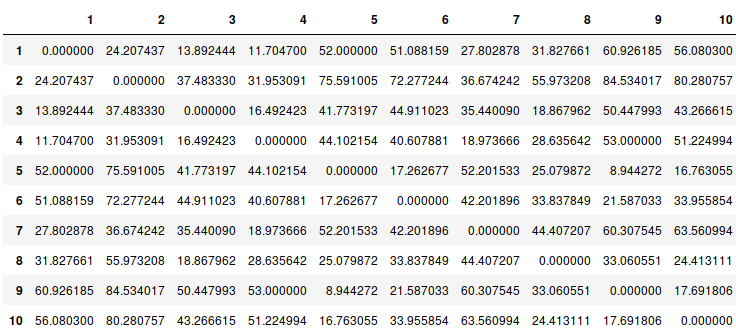
\includegraphics[scale=0.65]{table.png}
\end{figure}
\end{flushleft}

\begin{flushleft}
\\
\end{flushleft}


A travel egy 10 számból álló lista, amely a pontok meglátogatására utal. Feltételezzük, hogy zárt hurokra van szükség, így az utolsó pont autómatikusan csatlakozik az elsőhöz.


\begin{flushleft}
\begin{listings}
{\textit{travel = random.sample(range(10), 10);}
\end{listings}
\end{flushleft}


Elindítunk egy ciklust az adott értékekkel


\begin{flushleft}
\begin{listings}
{\textit{for tlp in numpy.logspace(0, 5, num = 100000)[::-1]:}
\end{listings}
\end{flushleft}


Két pont véletlenszerű cseréjével új új utat képzünk. Úgy valósítom meg, hogy választok két számot az i-t és a j-t. Összeállítom a newTravel-t a régi travel másolásával az i indexig, majd összefűzöm a j-edik travelel-t és egészen folytatom addig, amíg a j nem éri el az i-edik pontot, majd befejezem a travel többi részét.


\begin{flushleft}
\begin{listings}
{\textit{[i, j] = sorted(random.sample(range(10), 2)); \\
newTravel = travel[:i] + travel[j:j + 1] + travel[i + 1:j] + travel[i:i + 1] + travel[j + 1:];}
\end{listings}
\end{flushleft}


Ha az if értéke igaz akkor a travel megkapja a newTravel értékét, az előzöekben említett csere miatt ez már változott. Az elképzelés az, hogy minimalizálni szeretnénk a pontok közti távolságok költségének összegét. Ehhez a Gibb-s faktor-t használtam fel, aminek lényege, az új állapotba való átmenet valószínűsége. Csak az i-edik és j-edik pontok közötti távolságokat szükséges összegezni, mivel a többi távolság ugyanaz mint a travel-ben mint a newTravel-ben egyaránt. Ha a faktor > 1 akkor az új költség alacsonyabb, travel megkapja a newTravel értékét.


\begin{flushleft}

{\textit{traveld = sum([math.sqrt(sum( [(points[travel[(k + 1) \% 10]][d] - points[travel[k \% 10]][d]) **  2 for d in [0, 1]])) for k in [j, j - 1, i, i - 1]]) \\
    newTraveld = sum([math.sqrt(sum([(points[newTravel[(k + 1) \% 10]][d] - points[newTravel[k \% 10]][d]) ** 2 for d in [0, 1]])) for k in [j, j - 1, i, i - 1]]) \\
    if math.exp((traveld - newTraveld) / tlp) > random.random(): \\
        travel = copy.copy(newTravel);}

       
\end{flushleft}        


Az algoritmus végeztével már csak meg kell jeleníteni a kívánt pontokat, ez kirajzol egy gráfot, amely optimális utat ad. Ehhez a pyplot libary-t használtam


\begin{flushleft}
\begin{listings}
{\textit{plt.plot([points[travel[i \% 10]][0] for i in range(11)], [points[travel[i \% 10]][1] for i in range(11)], 'xb-'); \\
plt.show()}
\end{listings}
\end{flushleft}

A következő gráfok megmutatják a kívánt utat vároksok száma szerint. Mivel véletlenszerű számok összehasonlításán alapszik az algoritmus ezáltal az összehasonlítások száma igen magas, viszont stagnál bizonyos értékek között.

\begin{flushleft}
5 város esetén \\
Összehasonlítások száma: 74 434
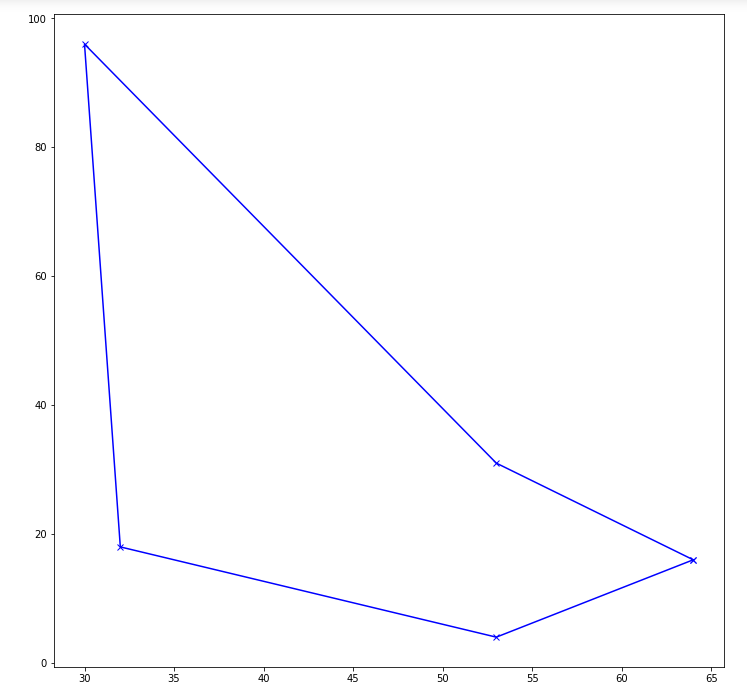
\includegraphics[scale=0.4]{5.png}
\end{flushleft}

\begin{flushleft}
10 város esetén \\
Összehasonlítások száma: 68 594
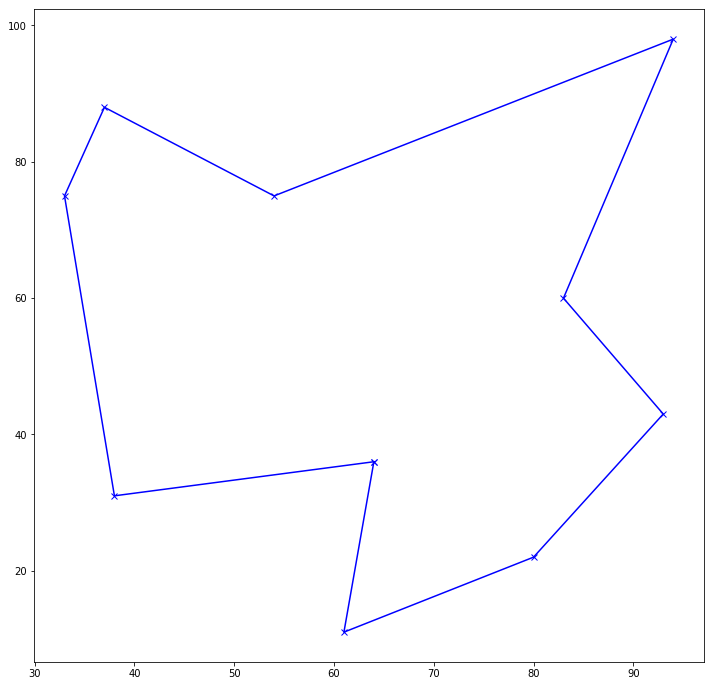
\includegraphics[scale=0.4]{10.png}
\end{flushleft}

\begin{flushleft}
15 város esetén \\
Összehasonlítások száma: 66 672
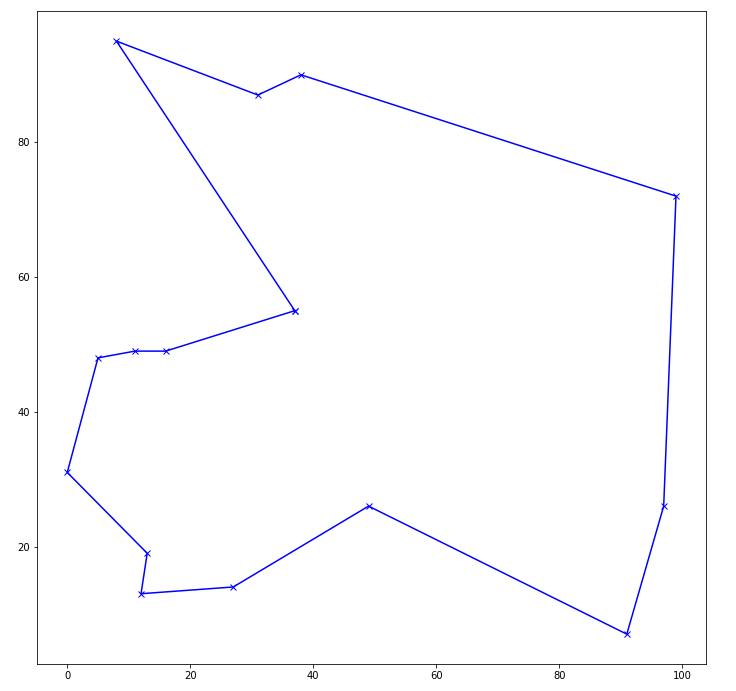
\includegraphics[scale=0.4]{15.png}
\end{flushleft}

\begin{flushleft}
20 város esetén \\
Összehasonlítások száma: 65 265
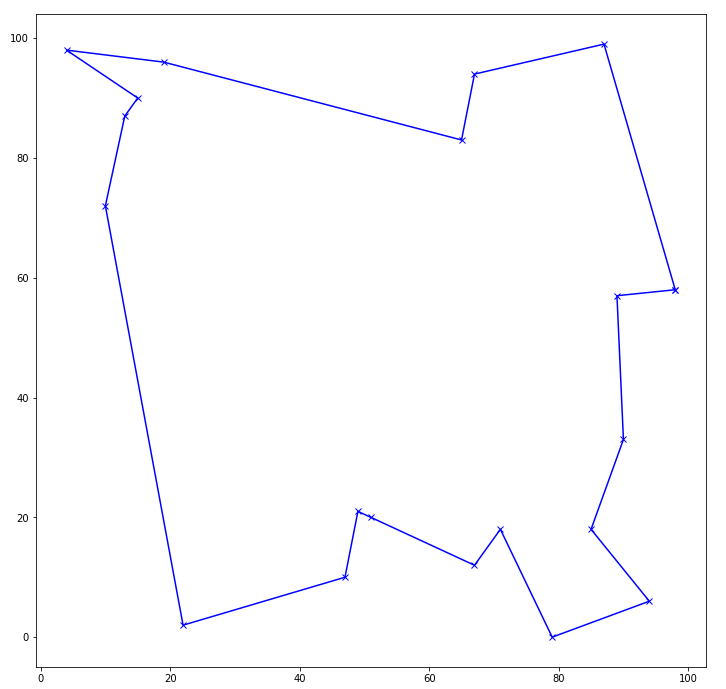
\includegraphics[scale=0.4]{20.png}
\end{flushleft}

\begin{flushleft}
25 város esetén \\
Összehasonlítások száma: 67 865
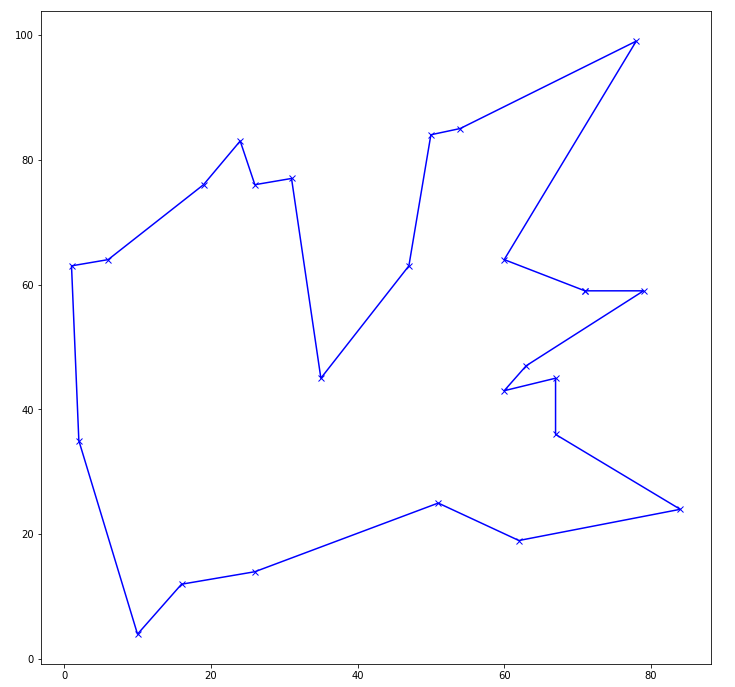
\includegraphics[scale=0.4]{25.png}
\end{flushleft}

\begin{flushleft}
30 város esetén \\
Összehasonlítások száma: 65 324
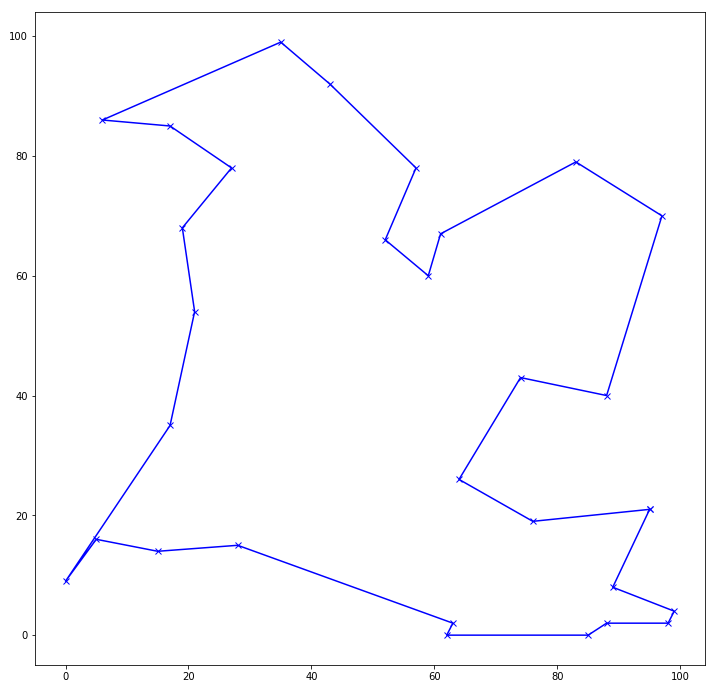
\includegraphics[scale=0.4]{30.png}
\end{flushleft}

\begin{flushleft}
35 város esetén \\
Összehasonlítások száma: 67 230
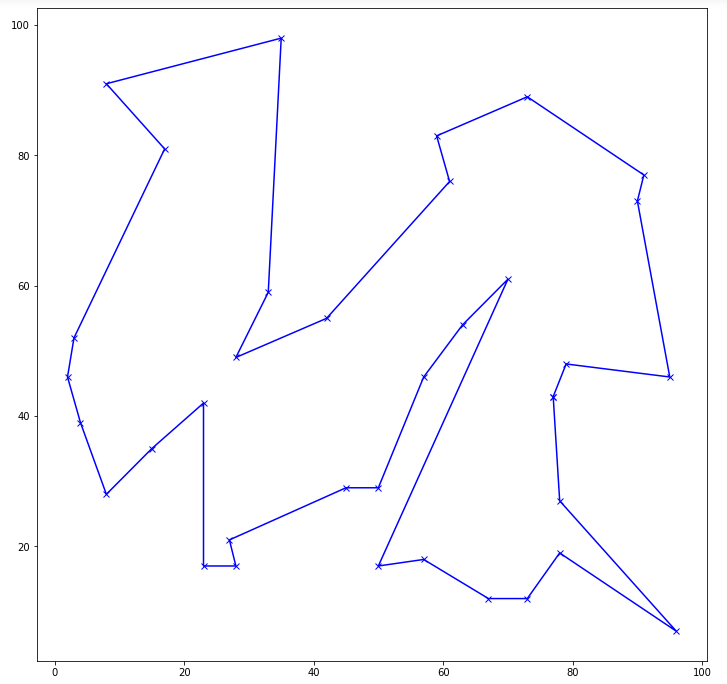
\includegraphics[scale=0.4]{35.png}
\end{flushleft}

\begin{flushleft}
40 város esetén \\
Összehasonlítások száma: 66 008
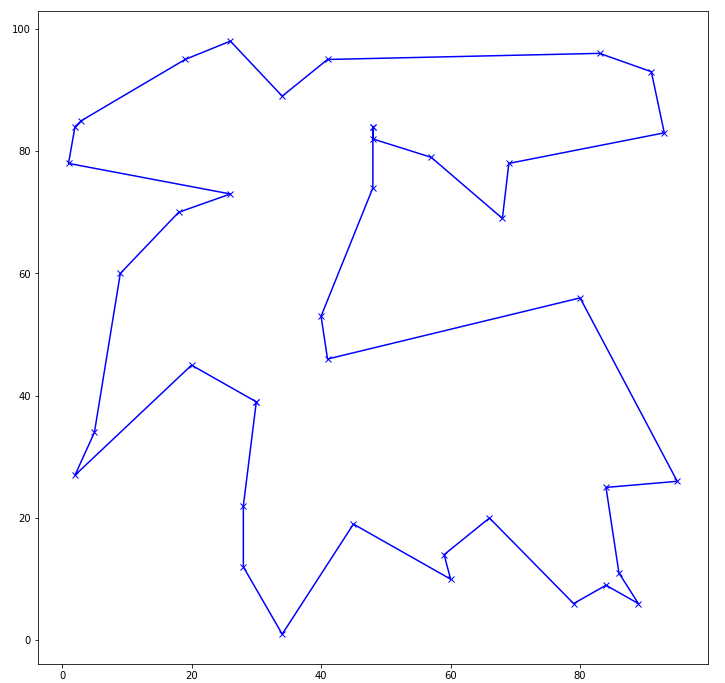
\includegraphics[scale=0.4]{40.png}
\end{flushleft}

Több lefuttatott teszt után is megfgyelhető, hogy az összehasonlítások száma 65 ezer és 75 ezer között mözög. Egytől egyig a legoptimálisabb utat adták

\end{document}